% Options for packages loaded elsewhere
\PassOptionsToPackage{unicode}{hyperref}
\PassOptionsToPackage{hyphens}{url}
\PassOptionsToPackage{dvipsnames,svgnames*,x11names*}{xcolor}
%
\documentclass[
  10pt,
]{article}
\usepackage{lmodern}
\usepackage{setspace}
\usepackage{amssymb,amsmath}
\usepackage{ifxetex,ifluatex}
\ifnum 0\ifxetex 1\fi\ifluatex 1\fi=0 % if pdftex
  \usepackage[T1]{fontenc}
  \usepackage[utf8]{inputenc}
  \usepackage{textcomp} % provide euro and other symbols
\else % if luatex or xetex
  \usepackage{unicode-math}
  \defaultfontfeatures{Scale=MatchLowercase}
  \defaultfontfeatures[\rmfamily]{Ligatures=TeX,Scale=1}
  \setmainfont[]{DejaVu Serif}
  \setmonofont[]{DejaVu Sans Mono}
\fi
% Use upquote if available, for straight quotes in verbatim environments
\IfFileExists{upquote.sty}{\usepackage{upquote}}{}
\IfFileExists{microtype.sty}{% use microtype if available
  \usepackage[]{microtype}
  \UseMicrotypeSet[protrusion]{basicmath} % disable protrusion for tt fonts
}{}
\makeatletter
\@ifundefined{KOMAClassName}{% if non-KOMA class
  \IfFileExists{parskip.sty}{%
    \usepackage{parskip}
  }{% else
    \setlength{\parindent}{0pt}
    \setlength{\parskip}{6pt plus 2pt minus 1pt}}
}{% if KOMA class
  \KOMAoptions{parskip=half}}
\makeatother
\usepackage{xcolor}
\IfFileExists{xurl.sty}{\usepackage{xurl}}{} % add URL line breaks if available
\IfFileExists{bookmark.sty}{\usepackage{bookmark}}{\usepackage{hyperref}}
\hypersetup{
  colorlinks=true,
  linkcolor=red,
  filecolor=red,
  citecolor=red,
  urlcolor=red,
  pdfcreator={LaTeX via pandoc}}
\urlstyle{same} % disable monospaced font for URLs
\usepackage[margin=1cm,top=1cm,bottom=1cm,left=1cm,right=1cm,includeheadfoot]{geometry}
\usepackage{listings}
\newcommand{\passthrough}[1]{#1}
\lstset{defaultdialect=[5.3]Lua}
\lstset{defaultdialect=[x86masm]Assembler}
\usepackage{longtable,booktabs}
% Correct order of tables after \paragraph or \subparagraph
\usepackage{etoolbox}
\makeatletter
\patchcmd\longtable{\par}{\if@noskipsec\mbox{}\fi\par}{}{}
\makeatother
% Allow footnotes in longtable head/foot
\IfFileExists{footnotehyper.sty}{\usepackage{footnotehyper}}{\usepackage{footnote}}
\makesavenoteenv{longtable}
\usepackage{graphicx}
\makeatletter
\def\maxwidth{\ifdim\Gin@nat@width>\linewidth\linewidth\else\Gin@nat@width\fi}
\def\maxheight{\ifdim\Gin@nat@height>\textheight\textheight\else\Gin@nat@height\fi}
\makeatother
% Scale images if necessary, so that they will not overflow the page
% margins by default, and it is still possible to overwrite the defaults
% using explicit options in \includegraphics[width, height, ...]{}
\setkeys{Gin}{width=\maxwidth,height=\maxheight,keepaspectratio}
% Set default figure placement to htbp
\makeatletter
\def\fps@figure{htbp}
\makeatother
\setlength{\emergencystretch}{3em} % prevent overfull lines
\providecommand{\tightlist}{%
  \setlength{\itemsep}{0pt}\setlength{\parskip}{0pt}}
\setcounter{secnumdepth}{3}
% Enable graphics inclusion and ensure figure numbering works
\usepackage{graphicx}
\renewcommand{\figurename}{Figure}

% Configure fonts for Unicode support with fallbacks
\usepackage{newunicodechar}
\newunicodechar{⁴}{\textsuperscript{4}}
\newunicodechar{₄}{\textsubscript{4}}

% Enhanced code block styling for better contrast and readability
\usepackage{fancyvrb}
\usepackage{xcolor}
\usepackage{listings}

% Define custom colors for code blocks
\definecolor{codebg}{RGB}{245, 245, 245}      % Light gray background
\definecolor{codeborder}{RGB}{200, 200, 200}  % Medium gray border
\definecolor{codefg}{RGB}{50, 50, 50}         % Dark gray text

% Configure Verbatim environment for inline code
\DefineVerbatimEnvironment{Verbatim}{Verbatim}{%
    fontsize=\small,
    frame=single,
    framerule=0.5pt,
    framesep=3pt,
    rulecolor=\color{codeborder},
    bgcolor=\color{codebg},
    fgcolor=\color{codefg}
}

% Configure code block styling
\DefineVerbatimEnvironment{Highlighting}{Verbatim}{%
    fontsize=\footnotesize,
    frame=single,
    framerule=0.5pt,
    framesep=5pt,
    rulecolor=\color{codeborder},
    bgcolor=\color{codebg},
    fgcolor=\color{codefg}
}

% Style inline code with \texttt
\renewcommand{\texttt}[1]{%
    \colorbox{codebg}{\color{codefg}\ttfamily #1}%
}

% Configure listings package for code blocks
\lstset{
    backgroundcolor=\color{codebg},
    basicstyle=\footnotesize\ttfamily\color{codefg},
    breakatwhitespace=false,
    breaklines=true,
    captionpos=b,
    commentstyle=\color{codefg},
    deletekeywords={...},
    escapeinside={\%*}{*)},
    extendedchars=true,
    frame=single,
    framerule=0.5pt,
    framesep=5pt,
    keepspaces=true,
    keywordstyle=\color{codefg},
    language=Python,
    morekeywords={*,...},
    numbers=left,
    numbersep=5pt,
    numberstyle=\tiny\color{codefg},
    rulecolor=\color{codeborder},
    showspaces=false,
    showstringspaces=false,
    showtabs=false,
    stepnumber=1,
    stringstyle=\color{codefg},
    tabsize=2,
    title=\lstname
}

% Override any Pandoc default lstset configurations
\AtBeginDocument{
    \lstset{
        backgroundcolor=\color{codebg},
        basicstyle=\footnotesize\ttfamily\color{codefg},
        frame=single,
        framerule=0.5pt,
        framesep=5pt,
        rulecolor=\color{codeborder},
        numbers=left,
        numbersep=5pt,
        numberstyle=\tiny\color{codefg}
    }
}

% Configure hyperref colors consistently
\AtBeginDocument{
% Override pandoc's hidelinks setting with consistent options
\hypersetup{
    colorlinks=true,
    allcolors=red,
    linkcolor=red,
    urlcolor=red,
    citecolor=red,
    filecolor=red,
    menucolor=red,
    linktoc=all
}
}

% Simple page break support for document structure

\title{Quadray Analytical Details and Methods}
\author{Daniel Ari Friedman\\ ORCID: 0000-0001-6232-9096\\ Email: daniel@activeinference.institute\\ DOI: 10.5281/zenodo.16887800}
\date{August 16, 2025}

\begin{document}
\maketitle

{
\hypersetup{linkcolor=black}
\setcounter{tocdepth}{3}
\tableofcontents
}
\setstretch{1.0}
\hypertarget{quadray-analytical-details-and-methods}{%
\section{Quadray Analytical Details and
Methods}\label{quadray-analytical-details-and-methods}}

\hypertarget{overview}{%
\subsection{Overview}\label{overview}}

This section provides detailed analytical methods for working with
Quadray coordinates, including coordinate conventions, volume
calculations, and optimization approaches. We emphasize the distinction
between different 4D frameworks and provide practical computational
methods.

\hypertarget{mathematical-foundations}{%
\subsection{Mathematical Foundations}\label{mathematical-foundations}}

The methods presented here rest on three interconnected mathematical
frameworks. For comprehensive definitions, see
\href{02_4d_namespaces.md}{Section 2: 4D Namespaces}.

\hypertarget{framework-distinctions}{%
\subsubsection{Framework Distinctions}\label{framework-distinctions}}

\begin{itemize}
\tightlist
\item
  \textbf{Coxeter.4D}: Euclidean 4D geometry with standard metric tensor
  and volume forms
\item
  \textbf{Einstein.4D}: Minkowski spacetime with indefinite metric for
  information geometry analogies\\
\item
  \textbf{Fuller.4D}: Synergetics/Quadray coordinates with integer
  lattice constraints and IVM unit conventions
\end{itemize}

\hypertarget{key-mathematical-principles}{%
\subsubsection{Key Mathematical
Principles}\label{key-mathematical-principles}}

\begin{itemize}
\tightlist
\item
  \textbf{Integer volume quantization}: Lattice constraints ensure
  tetrahedral volumes are exact integers in IVM units
\item
  \textbf{Coordinate system bridges}: Linear transformations between
  Fuller.4D and Coxeter.4D preserve geometric relationships
\item
  \textbf{Information geometry}: Fisher metric provides Riemannian
  structure for optimization on parameter manifolds
\item
  \textbf{Exact arithmetic}: Bareiss algorithm ensures determinant
  calculations remain exact for integer inputs
\end{itemize}

\hypertarget{implementation-strategy}{%
\subsubsection{Implementation Strategy}\label{implementation-strategy}}

All mathematical concepts are implemented with: - \textbf{Exact
arithmetic} where possible (integer determinants, symbolic computation)
- \textbf{Numerical stability} for floating-point operations (ridge
regularization, condition number monitoring) - \textbf{Cross-validation}
between different formulations (Ace 5×5 vs Cayley--Menger, native vs
bridging approaches) - \textbf{Comprehensive testing} ensuring
mathematical correctness across edge cases

\hypertarget{framework-integration}{%
\subsection{Framework Integration}\label{framework-integration}}

The three 4D frameworks serve distinct but complementary roles in our
implementation:

\begin{itemize}
\item
  \textbf{Coxeter.4D provides the container}: Euclidean 4D space serves
  as the mathematical foundation for volume calculations, distance
  metrics, and geometric transformations. When we compute volumes via
  Cayley--Menger determinants or XYZ coordinate determinants, we operate
  in this framework.
\item
  \textbf{Einstein.4D provides the analogy}: The Minkowski metric
  structure inspires our information geometry approach, where the Fisher
  information matrix acts as a Riemannian metric on parameter space.
  Natural gradient descent follows geodesics on this information
  manifold, analogous to how particles follow geodesics in spacetime.
\item
  \textbf{Fuller.4D provides the constraints}: The Quadray coordinate
  system and IVM lattice impose integer constraints that enable exact
  arithmetic and discrete optimization. The synergetics unit conventions
  (regular tetrahedron volume = 1) create a quantized geometry where
  volumes are exact integers.
\end{itemize}

This multi-framework approach allows us to: 1. Use standard Euclidean
methods for volume calculations where relevant or already in use
(Coxeter.4D) 2. Apply information geometry principles for geodesic
optimization (Einstein.4D analogy)\\
3. Maintain exact arithmetic in the Isotropic Vector Matrix (IVM)
setting through integer lattice constraints (Fuller.4D) 4. Bridge and
swap among frameworks via coordinate transformations and unit
conversions

\hypertarget{fuller.4d-coordinates-and-normalization}{%
\subsection{Fuller.4D Coordinates and
Normalization}\label{fuller.4d-coordinates-and-normalization}}

\begin{itemize}
\tightlist
\item
  Quadray vector q = (a,b,c,d), a,b,c,d ≥ 0, with at least one
  coordinate zero under normalization.
\item
  Projective normalization can add/subtract (k,k,k,k) without changing
  direction; choose k to enforce non-negativity and one zero minimum.
\item
  Isotropic Vector Matrix (IVM): integer quadrays describe CCP sphere
  centers; the 12 permutations of \{2,1,1,0\} form the cuboctahedron
  (vector equilibrium).

  \begin{itemize}
  \tightlist
  \item
    Integer-coordinate models: assigning unit IVM tetravolume to the
    regular tetrahedron yields integer coordinates for several familiar
    polyhedra (inverse tetrahedron, cube, octahedron, rhombic
    dodecahedron, cuboctahedron) when expressed as linear combinations
    of the four quadray basis vectors. See overview:
    \href{https://en.wikipedia.org/wiki/Quadray_coordinates}{Quadray
    coordinates}.
  \end{itemize}
\end{itemize}

\hypertarget{conversions-and-vector-operations-quadray-cartesian-fuller.4d-coxeter.4dxyz}{%
\subsection{Conversions and Vector Operations: Quadray ↔ Cartesian
(Fuller.4D ↔
Coxeter.4D/XYZ)}\label{conversions-and-vector-operations-quadray-cartesian-fuller.4d-coxeter.4dxyz}}

\begin{itemize}
\tightlist
\item
  \textbf{Embedding conventions} determine the linear maps between
  Quadray (Fuller.4D) and Cartesian XYZ (a 3D slice or embedding aligned
  with Coxeter.4D conventions).
\item
  \textbf{References}: Urner provides practical conversion write-ups and
  matrices; see:

  \begin{itemize}
  \tightlist
  \item
    Quadrays and XYZ:
    \href{https://www.grunch.net/synergetics/quadxyz.html}{Urner --
    Quadrays and XYZ}
  \item
    Introduction with examples:
    \href{https://www.grunch.net/synergetics/quadintro.html}{Urner --
    Quadray intro}
  \end{itemize}
\item
  \textbf{Implementation}: choose a fixed tetrahedral embedding;
  construct a 3×4 matrix M that maps (a,b,c,d) to (x,y,z), respecting
  A,B,C,D directions to tetra vertices. The inverse map can be defined
  up to projective normalization (adding (k,k,k,k)). When comparing
  volumes, use the \passthrough{\lstinline!S3=\\sqrt\{9/8\}!} scale to
  convert XYZ (Euclidean) volumes to IVM (Fuller.4D) units.
\item
  \textbf{Vector view}: treat \passthrough{\lstinline!q!} as a vector
  with magnitude and direction; define dot products and norms by pushing
  to XYZ via \passthrough{\lstinline!M!}.
\end{itemize}

\hypertarget{integer-coordinate-constructions-compact-derivation-box}{%
\subsubsection{Integer-coordinate constructions (compact derivation
box)}\label{integer-coordinate-constructions-compact-derivation-box}}

\begin{itemize}
\tightlist
\item
  Under the synergetics convention (unit regular tetrahedron has
  tetravolume 1), many familiar solids admit Quadray integer
  coordinates. For example, the octahedron at the same edge length has
  tetravolume 4, and its vertices can be formed as integer linear
  combinations of the four axes A,B,C,D subject to the Quadray
  normalization rule.
\item
  The cuboctahedron (vector equilibrium) arises as the shell of the 12
  nearest IVM neighbors given by the permutations of \((2,1,1,0)\). The
  rhombic dodecahedron (tetravolume 6) is the Voronoi cell of the
  FCC/CCP packing centered at the origin under the same embedding.
\item
  See the following figure for a schematic summary of these
  relationships.
\end{itemize}

\begin{longtable}[]{@{}lll@{}}
\toprule
\begin{minipage}[b]{0.30\columnwidth}\raggedright
Object\strut
\end{minipage} & \begin{minipage}[b]{0.30\columnwidth}\raggedright
Quadray construction (sketch)\strut
\end{minipage} & \begin{minipage}[b]{0.30\columnwidth}\raggedright
IVM volume\strut
\end{minipage}\tabularnewline
\midrule
\endhead
\begin{minipage}[t]{0.30\columnwidth}\raggedright
Regular tetrahedron\strut
\end{minipage} & \begin{minipage}[t]{0.30\columnwidth}\raggedright
Vertices \passthrough{\lstinline!o=(0,0,0,0)!},
\passthrough{\lstinline!p=(2,1,0,1)!},
\passthrough{\lstinline!q=(2,1,1,0)!},
\passthrough{\lstinline!r=(2,0,1,1)!}\strut
\end{minipage} & \begin{minipage}[t]{0.30\columnwidth}\raggedright
1\strut
\end{minipage}\tabularnewline
\begin{minipage}[t]{0.30\columnwidth}\raggedright
Cube (same edge)\strut
\end{minipage} & \begin{minipage}[t]{0.30\columnwidth}\raggedright
Union of 3 mutually orthogonal rhombic belts wrapped on the tetra frame;
edges tracked by XYZ embedding; compare the following figure\strut
\end{minipage} & \begin{minipage}[t]{0.30\columnwidth}\raggedright
3\strut
\end{minipage}\tabularnewline
\begin{minipage}[t]{0.30\columnwidth}\raggedright
Octahedron (same edge)\strut
\end{minipage} & \begin{minipage}[t]{0.30\columnwidth}\raggedright
Convex hull of mid-edges of the tetra frame (pairwise axis sums
normalized)\strut
\end{minipage} & \begin{minipage}[t]{0.30\columnwidth}\raggedright
4\strut
\end{minipage}\tabularnewline
\begin{minipage}[t]{0.30\columnwidth}\raggedright
Rhombic dodecahedron\strut
\end{minipage} & \begin{minipage}[t]{0.30\columnwidth}\raggedright
Voronoi cell of FCC/CCP packing at origin (dual to cuboctahedron)\strut
\end{minipage} & \begin{minipage}[t]{0.30\columnwidth}\raggedright
6\strut
\end{minipage}\tabularnewline
\begin{minipage}[t]{0.30\columnwidth}\raggedright
Cuboctahedron (vector equilibrium)\strut
\end{minipage} & \begin{minipage}[t]{0.30\columnwidth}\raggedright
Shell of the 12 nearest IVM neighbors: permutations of
\passthrough{\lstinline!(2,1,1,0)!}\strut
\end{minipage} & \begin{minipage}[t]{0.30\columnwidth}\raggedright
20\strut
\end{minipage}\tabularnewline
\begin{minipage}[t]{0.30\columnwidth}\raggedright
Truncated octahedron\strut
\end{minipage} & \begin{minipage}[t]{0.30\columnwidth}\raggedright
Archimedean solid with 6 square and 8 hexagonal faces; space-filling
tiling\strut
\end{minipage} & \begin{minipage}[t]{0.30\columnwidth}\raggedright
20\strut
\end{minipage}\tabularnewline
\bottomrule
\end{longtable}

Small coordinate examples (subset):

\begin{itemize}
\tightlist
\item
  Cuboctahedron neighbors (representatives):
  \passthrough{\lstinline!(2,1,1,0)!},
  \passthrough{\lstinline!(2,1,0,1)!},
  \passthrough{\lstinline!(2,0,1,1)!},
  \passthrough{\lstinline!(1,2,1,0)!}; the full shell is all distinct
  permutations.
\item
  Tetrahedron:
  \passthrough{\lstinline![(0,0,0,0), (2,1,0,1), (2,1,1,0), (2,0,1,1)]!}.
\end{itemize}

Short scripts:

\begin{lstlisting}[language=bash]
python3 quadmath/scripts/polyhedra_quadray_constructions.py
\end{lstlisting}

Programmatic check (neighbors, equal radii, adjacency):

\begin{lstlisting}[language=Python]
import numpy as np
from examples import example_cuboctahedron_vertices_xyz

xyz = np.array(example_cuboctahedron_vertices_xyz())
r = np.linalg.norm(xyz[0])
assert np.allclose(np.linalg.norm(xyz, axis=1), r)

# Touching neighbors have separation 2r
touch = []
for i in range(len(xyz)):
    for j in range(i+1, len(xyz)):
        d = np.linalg.norm(xyz[i] - xyz[j])
        if abs(d - 2*r) / (2*r) < 0.05:
            touch.append((i, j))
assert len(touch) > 0
\end{lstlisting}

\hypertarget{example-vertex-lists-and-volume-checks-illustrative}{%
\subsubsection{Example vertex lists and volume checks
(illustrative)}\label{example-vertex-lists-and-volume-checks-illustrative}}

The following snippets use canonical IVM neighbor points (permutations
of \((2,1,1,0)\)) to illustrate simple decompositions consistent with
synergetics volumes. Each tetra volume is computed via
\passthrough{\lstinline!ace\_tetravolume\_5x5!} and summed.

Octahedron (V = 4) as four unit IVM tetras around the origin:

\begin{lstlisting}[language=Python]
from quadray import Quadray, ace_tetravolume_5x5

o = Quadray(0,0,0,0)
T = [
    (Quadray(2,1,0,1), Quadray(2,1,1,0), Quadray(2,0,1,1)),
    (Quadray(1,2,0,1), Quadray(1,2,1,0), Quadray(0,2,1,1)),
    (Quadray(1,1,2,0), Quadray(1,0,2,1), Quadray(0,1,2,1)),
    (Quadray(2,0,1,1), Quadray(1,2,0,1), Quadray(0,1,2,1)),  # representative variant
]
V_oct = sum(ace_tetravolume_5x5(o, a, b, c) for (a,b,c) in T)
\end{lstlisting}

Cube (V = 3) as three unit IVM tetras (orthant-like around the origin):

\begin{lstlisting}[language=Python]
from quadray import Quadray, ace_tetravolume_5x5

o = Quadray(0,0,0,0)
triples = [
    (Quadray(2,1,0,1), Quadray(2,1,1,0), Quadray(2,0,1,1)),
    (Quadray(1,2,0,1), Quadray(1,2,1,0), Quadray(0,2,1,1)),
    (Quadray(1,1,2,0), Quadray(1,0,2,1), Quadray(0,1,2,1)),
]
V_cube = sum(ace_tetravolume_5x5(o, a, b, c) for (a,b,c) in triples)
\end{lstlisting}

Notes.

\begin{itemize}
\tightlist
\item
  These decompositions are illustrative and use canonical IVM neighbor
  triples that produce unit tetras under
  \passthrough{\lstinline!ace\_tetravolume\_5x5!}. Other equivalent
  tilings are possible.
\item
  Volumes are invariant to adding \((k,k,k,k)\) to each vertex of a
  tetra (projective normalization), which the 5×5 determinant respects.
\end{itemize}

\hypertarget{sec:integer_volume}{%
\subsection{Integer Volume Quantization}\label{sec:integer_volume}}

For a tetrahedron with vertices P₀..P₃ in the Quadray integer lattice
(Fuller.4D), see Eq. \eqref{eq:lattice_det} in the equations appendix.

\begin{itemize}
\tightlist
\item
  With integer coordinates, the determinant is integer; lattice
  tetrahedra yield integer volumes.
\item
  Unit conventions: regular tetrahedron volume = 1 (synergetics).
\end{itemize}

Notes.

\begin{itemize}
\tightlist
\item
  \(P_0,\ldots,P_3\) are tetrahedron vertices in Quadray coordinates.
\item
  \(V\) is the Euclidean volume measured in IVM tetra-units; the \(1/6\)
  factor converts the parallelepiped determinant to a tetra volume.
\item
  Background and variations are discussed under Tetrahedron volume
  formulas:
  \href{https://en.wikipedia.org/wiki/Tetrahedron\#Volume}{Tetrahedron
  -- volume}.
\end{itemize}

Tom Ace 5×5 determinant (tetravolume directly from quadrays), see Eq.
\eqref{eq:ace5x5} in the equations appendix.

This returns the same integer volumes for lattice tetrahedra. See the
implementation \passthrough{\lstinline!ace\_tetravolume\_5x5!}.

Notes.

\begin{itemize}
\tightlist
\item
  Rows correspond to the Quadray 4-tuples of the four vertices with a
  final affine column of ones; the last row enforces projective
  normalization.
\item
  The factor \(\tfrac{1}{4}\) returns tetravolumes in IVM units
  consistent with synergetics. See also
  \href{https://en.wikipedia.org/wiki/Quadray_coordinates}{Quadray
  coordinates}.
\end{itemize}

Equivalently, define the 5×5 matrix of quadray coordinates augmented
with an affine 1 as shown in Eq. \eqref{eq:ace5x5_expanded} in the
equations appendix.

Points vs vectors: subtracting points is shorthand for forming edge
vectors. We treat quadray 4-tuples as vectors from the origin;
differences like \((P_1-P_0)\) mean ``edge vectors,'' avoiding ambiguity
between ``points'' and ``vectors.''

Equivalently via Cayley--Menger determinant (Coxeter.4D/Euclidean
lengths)
(\href{https://en.wikipedia.org/wiki/Cayley\%E2\%80\%93Menger_determinant}{Cayley--Menger
determinant}), see Eq. \eqref{eq:cayley_menger} in the equations
appendix.

References:
\href{https://en.wikipedia.org/wiki/Cayley\%E2\%80\%93Menger_determinant}{Cayley--Menger
determinant}, lattice tetrahedra discussions in geometry texts; see also
\href{https://en.wikipedia.org/wiki/Tetrahedron\#Volume}{Tetrahedron --
volume}. Code: \passthrough{\lstinline!integer\_tetra\_volume!},
\passthrough{\lstinline!ace\_tetravolume\_5x5!}.

Notes.

\begin{itemize}
\tightlist
\item
  \textbf{Pairwise distances}: \(d_{ij}\) are Euclidean distances
  between vertices \(P_i\) and \(P_j\).
\item
  \textbf{Length-only formulation}: Cayley--Menger provides a
  length-only formula for simplex volumes, here specialized to
  tetrahedra; see the canonical reference above.
\end{itemize}

\begin{longtable}[]{@{}ll@{}}
\caption{Polyhedra tetravolumes in IVM units (edge length equal to the
unit tetra edge). \{\#tbl:polyhedra\_volumes\}}\tabularnewline
\toprule
Polyhedron (edge = tetra edge) & Volume (tetra-units)\tabularnewline
\midrule
\endfirsthead
\toprule
Polyhedron (edge = tetra edge) & Volume (tetra-units)\tabularnewline
\midrule
\endhead
Regular Tetrahedron & 1\tabularnewline
Cube & 3\tabularnewline
Octahedron & 4\tabularnewline
Rhombic Dodecahedron & 6\tabularnewline
Cuboctahedron (Vector Equilibrium) & 20\tabularnewline
Truncated Octahedron & 20\tabularnewline
\bottomrule
\end{longtable}

\hypertarget{distances-and-metrics}{%
\subsection{Distances and Metrics}\label{distances-and-metrics}}

Distance definitions depend on the chosen embedding and normalization.
For cross-references to information geometry, see
\href{08_equations_appendix.md\#eq:fim}{Eq. (FIM)} and
\href{08_equations_appendix.md\#eq:natgrad}{natural gradient} in the
Equations appendix.

\hypertarget{sec:xyz_conversion}{%
\subsection{XYZ determinant and S3
conversion}\label{sec:xyz_conversion}}

Given XYZ coordinates of tetrahedron vertices (x\_i, y\_i, z\_i), the
Euclidean volume is computed as shown in Eq. \eqref{eq:xyz_det} in the
equations appendix.

Convert to IVM units via \(V_{ivm} = S3 \cdot V_{xyz}\) with
\(S3=\sqrt{9/8}\). See background discussion under
\href{https://en.wikipedia.org/wiki/Tetrahedron\#Volume}{Tetrahedron --
volume}.

\hypertarget{alternative-volume-formulas}{%
\subsubsection{Alternative Volume
Formulas}\label{alternative-volume-formulas}}

\begin{itemize}
\item
  \textbf{Piero della Francesca (PdF) formula}, which consumes edge
  lengths and returns Euclidean volumes. See Eq. \eqref{eq:pdf} in the
  equations appendix.

  Convert to IVM units via \(V_{ivm} = S3 \cdot V_{xyz}\) with
  \(S3=\sqrt{9/8}\). See background discussion under
  \href{https://en.wikipedia.org/wiki/Tetrahedron\#Volume}{Tetrahedron
  -- volume}.
\item
  \textbf{Gerald de Jong (GdJ) formula}, which natively returns
  tetravolumes. See Eq. \eqref{eq:gdj} in the equations appendix.

  In Quadray coordinates, one convenient native form uses edge-vector
  differences and an integer-preserving determinant (agreeing with Ace
  5×5):

  where each column is formed from Quadray component differences of
  \(P_1-P_0\), \(P_2-P_0\), \(P_3-P_0\) projected to a 3D slice
  consistent with the synergetics convention; integer arithmetic is
  exact and the factor \(\tfrac{1}{4}\) produces IVM tetravolumes. See
  de Jong's Quadray notes and Urner's implementations for derivations
  (\href{https://en.wikipedia.org/wiki/Quadray_coordinates}{Quadray
  coordinates}).
\item
  Euclidean embedding distance via appropriate linear map from quadray
  to R³.
\item
  Information geometry metric: Fisher Information Matrix (FIM)

  \begin{itemize}
  \tightlist
  \item
    \(\mathrm{FIM}[i,j] = \mathbb{E}\big[\, \partial_{\theta_i} \log p(x;\theta)\,\partial_{\theta_j} \log p(x;\theta)\,\big]\)
  \item
    Acts as Riemannian metric; natural gradient uses FIM⁻¹ ∇θ L. See
    \href{https://en.wikipedia.org/wiki/Fisher_information}{Fisher
    information}.
  \end{itemize}
\end{itemize}

\hypertarget{fisher-geometry-in-quadray-space}{%
\subsection{Fisher Geometry in Quadray
Space}\label{fisher-geometry-in-quadray-space}}

\begin{itemize}
\tightlist
\item
  Symmetries of quadray lattices often induce near block-diagonal FIM.
\item
  Determinant and spectrum characterize conditioning and information
  concentration.
\end{itemize}

\hypertarget{practical-methods}{%
\subsection{Practical Methods}\label{practical-methods}}

\hypertarget{sec:tetravolumes_quadrays}{%
\subsection{Tetravolumes with
Quadrays}\label{sec:tetravolumes_quadrays}}

\begin{itemize}
\item
  The tetravolume of a tetrahedron with vertices given as Quadrays
  \passthrough{\lstinline!a,b,c,d!} can be computed directly from their
  4-tuples via the Tom Ace 5×5 determinant; see Eq. \eqref{eq:ace5x5}
  for the canonical form.
\item
  Unit regular tetrahedron from origin: with
  \passthrough{\lstinline!o=(0,0,0,0)!},
  \passthrough{\lstinline!p=(2,1,0,1)!},
  \passthrough{\lstinline!q=(2,1,1,0)!},
  \passthrough{\lstinline!r=(2,0,1,1)!}, we have
  \passthrough{\lstinline!V\_ivm(o,p,q,r)=1!}. Doubling each vector
  scales volume by 8, as expected.
\item
  Equivalent length-based formulas agree with the 5×5 determinant:

  \begin{itemize}
  \tightlist
  \item
    Cayley--Menger:
    \(288\,V^2 = \det\begin{pmatrix}0&1&1&1&1\\1&0&d_{01}^2&d_{02}^2&d_{03}^2\\1&d_{10}^2&0&d_{12}^2&d_{13}^2\\1&d_{20}^2&d_{21}^2&0&d_{23}^2\\1&d_{30}^2&d_{31}^2&d_{32}^2&0\end{pmatrix}\).
  \item
    Piero della Francesca (PdF) Heron-like formula (converted to IVM via
    \(S3 = \sqrt{9/8}\)).
  \end{itemize}

  Let edge lengths meeting at a vertex be \(a,b,c\), and the opposite
  edges be \(d,e,f\). The Euclidean volume satisfies

  Convert to IVM units via \(V_{ivm} = S3 \cdot V_{xyz}\) with
  \(S3=\sqrt{9/8}\). See background discussion under
  \href{https://en.wikipedia.org/wiki/Tetrahedron\#Volume}{Tetrahedron
  -- volume}.
\item
  Gerald de Jong (GdJ) formula, which natively returns tetravolumes.

  In Quadray coordinates, one convenient native form uses edge-vector
  differences and an integer-preserving determinant (agreeing with Ace
  5×5):

  where each column is formed from Quadray component differences of
  \(P_1-P_0\), \(P_2-P_0\), \(P_3-P_0\) projected to a 3D slice
  consistent with the synergetics convention; integer arithmetic is
  exact and the factor \(\tfrac{1}{4}\) produces IVM tetravolumes. See
  de Jong's Quadray notes and Urner's implementations for derivations
  (\href{https://en.wikipedia.org/wiki/Quadray_coordinates}{Quadray
  coordinates}).
\end{itemize}

\hypertarget{bridging-and-native-tetravolume-formulas}{%
\subsubsection{Bridging and native tetravolume
formulas}\label{bridging-and-native-tetravolume-formulas}}

\begin{itemize}
\tightlist
\item
  \textbf{Lengths (bridging)}: PdF and Cayley--Menger (CM) consume
  Cartesian lengths (XYZ) and produce Euclidean volumes; convert to IVM
  units via \(S3 = \sqrt{9/8}\).
\item
  \textbf{Quadray-native}: Gerald de Jong (GdJ) returns IVM tetravolumes
  directly (no XYZ bridge). Tom Ace's 5×5 coordinate formula is likewise
  native IVM. All agree numerically with CM+S3 on shared cases.
\end{itemize}

References and discussion: \href{https://flic.kr/p/2rn22en}{Urner --
Flickr diagram}. For computational implementations and educational
materials, see the \href{07_resources.md}{Resources} section.

Figure: automated comparison (native Ace 5×5 vs CM+S3) across small
examples (see script \passthrough{\lstinline!sympy\_formalisms.py!}).
The figure and source CSV/NPZ are in
\passthrough{\lstinline!quadmath/output/!}.

\begin{figure}
\centering
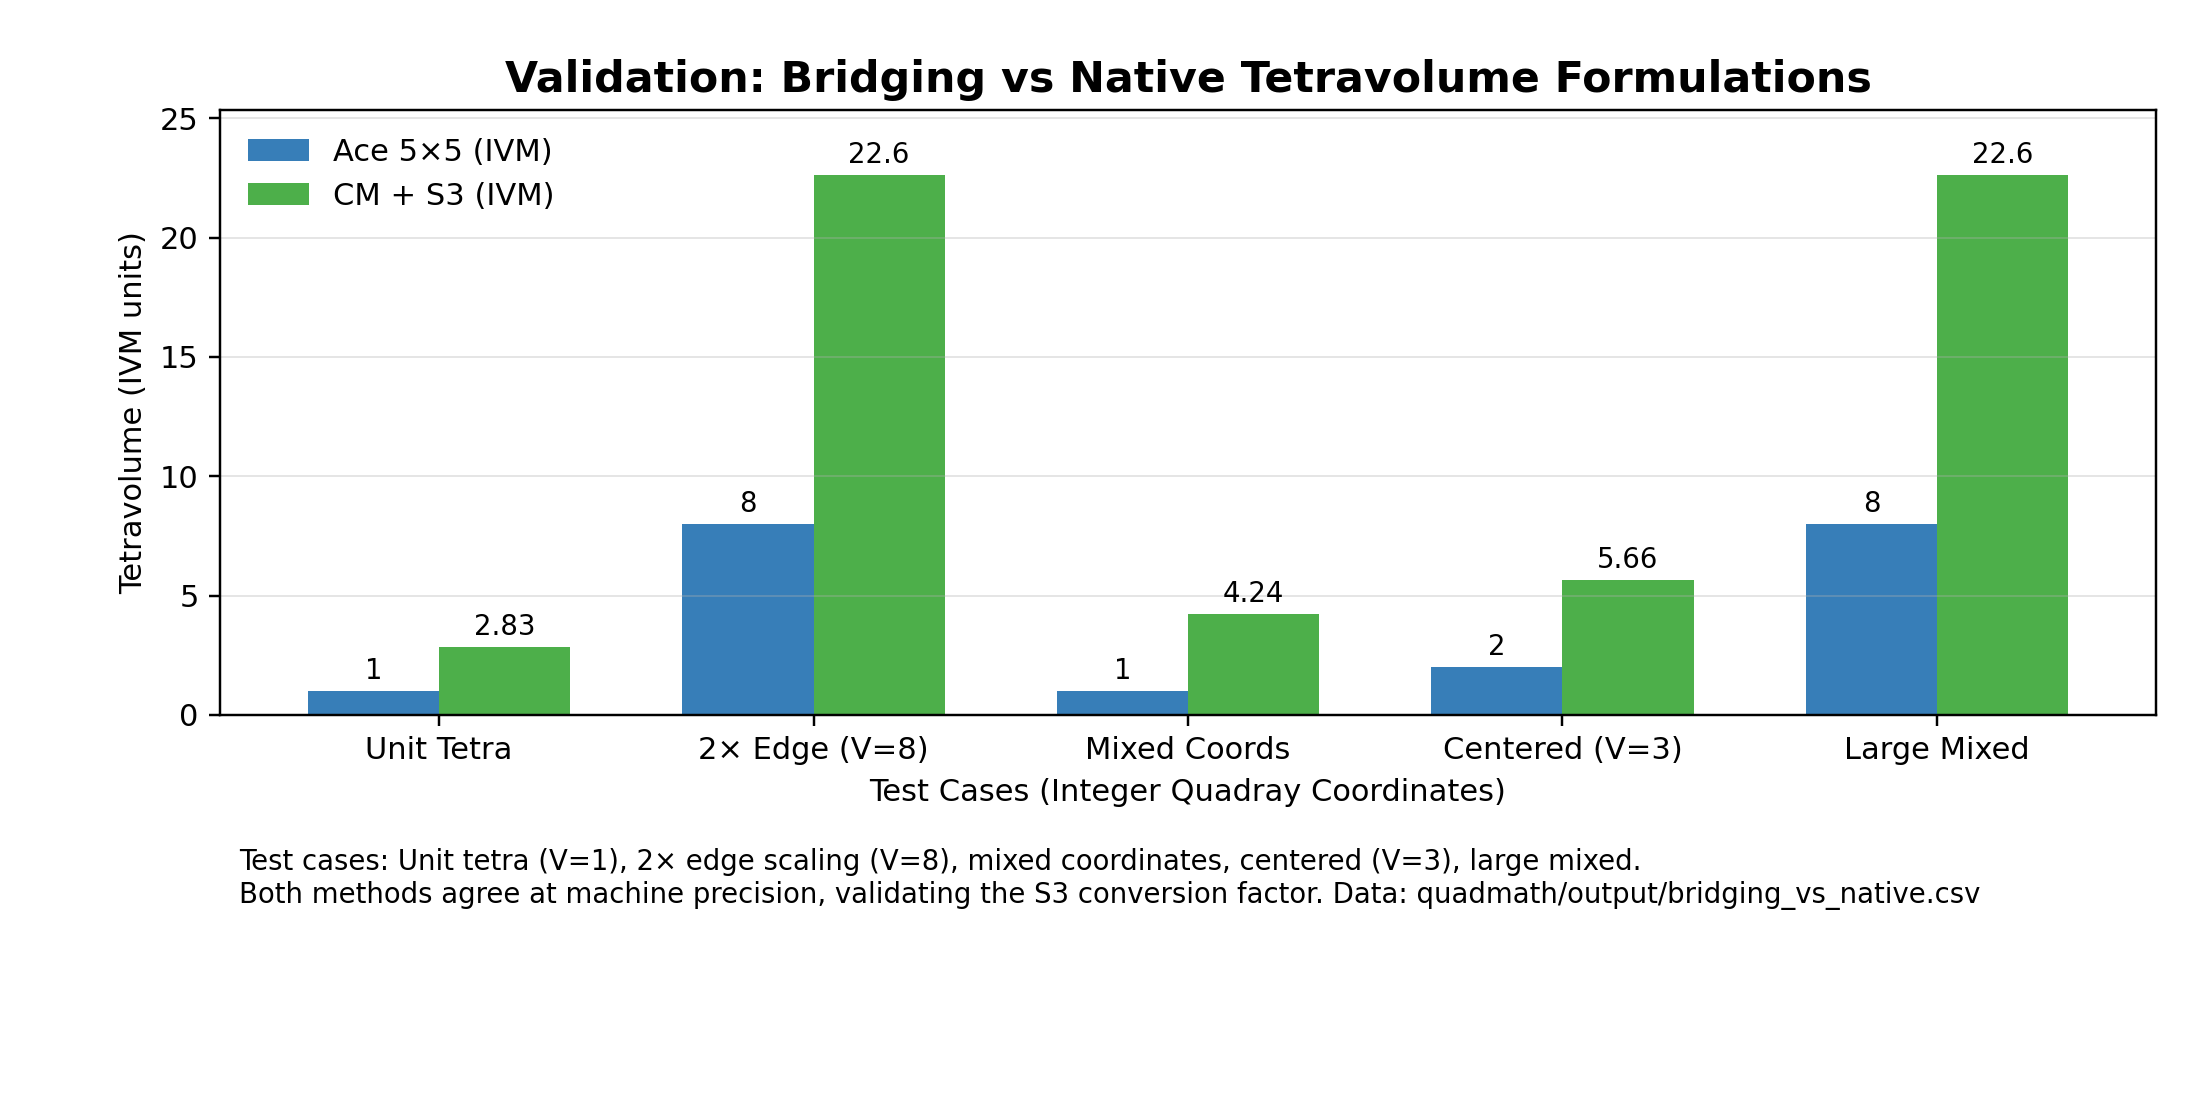
\includegraphics{../output/figures/bridging_vs_native.png}
\caption{\textbf{Validation of bridging vs native tetravolume
formulations across canonical examples}. This bar chart compares IVM
tetravolumes computed via two independent methods: the ``bridging''
approach using Cayley--Menger determinants on Euclidean edge lengths
converted to IVM units via the synergetics factor \(S3=\sqrt{9/8}\),
versus the ``native'' approach using Tom Ace's 5×5 determinant formula
that operates directly on Quadray coordinates without XYZ intermediates.
\textbf{Test cases}: Unit tetrahedron (V=1), 2× edge scaling (V=8),
mixed coordinate tetrahedron, centered tetrahedron (V=3), and large
mixed tetrahedron, all using integer Quadray coordinates.
\textbf{Results}: The overlapping bars demonstrate numerical agreement
at machine precision between the length-based Coxeter.4D approach
(Cayley--Menger + S3 conversion) and the coordinate-based Fuller.4D
approach (Ace 5×5), confirming the mathematical equivalence of these
formulations under synergetics unit conventions. Raw numerical data
saved as \passthrough{\lstinline!bridging\_vs\_native.csv!} for
reproducibility and further analysis.}
\end{figure}

\begin{figure}
\centering
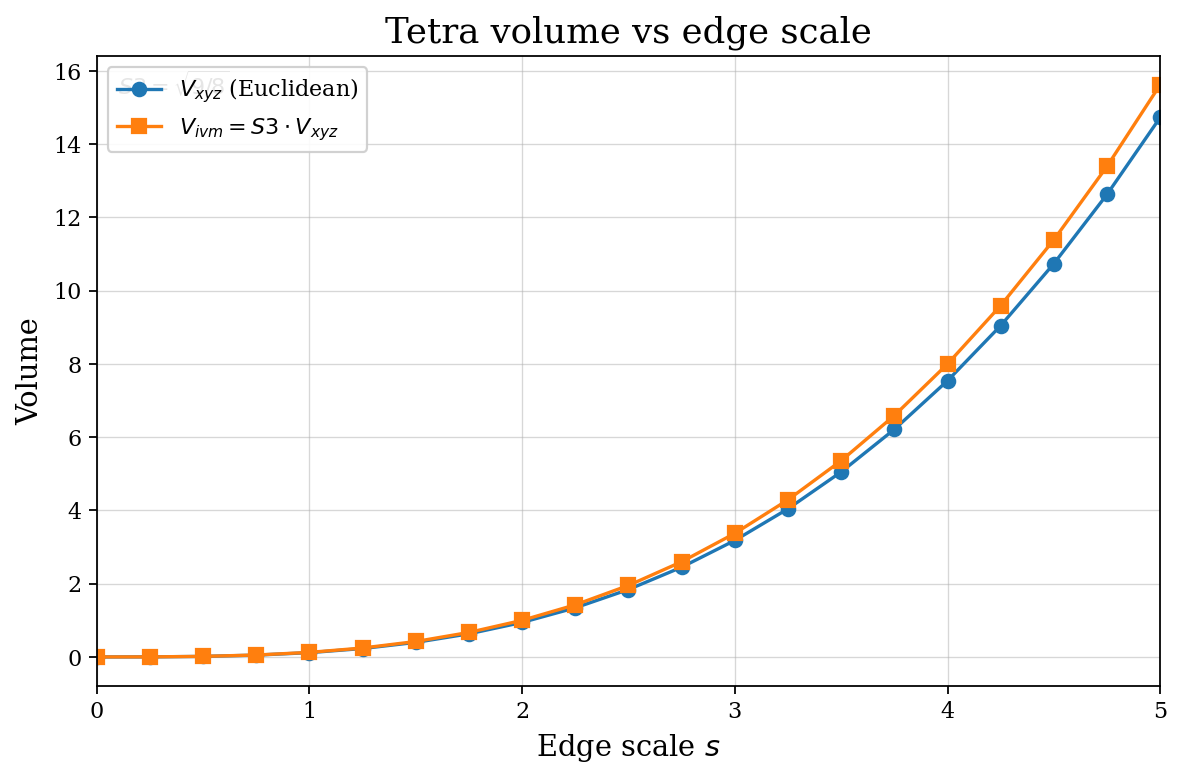
\includegraphics{../output/figures/volumes_scale_plot.png}
\caption{\textbf{Tetrahedron volume scaling relationships: Euclidean vs
IVM unit conventions}. This plot demonstrates the mathematical
relationship between edge length scaling and tetravolume under both
Euclidean (XYZ) and IVM (synergetics) unit conventions. \textbf{X-axis}:
Edge length scaling factor (0 to 5.0). \textbf{Y-axis}: Tetrahedron
volume in respective units. \textbf{Blue line (Euclidean)}: Volume
scales as the cube of edge length, following the standard
\(V = \frac{\sqrt{2}}{12} \cdot L^3\) relationship for regular
tetrahedra. \textbf{Orange line (IVM)}: Volume scales as the cube of
edge length but in IVM tetra-units, following
\(V_{ivm} = \frac{1}{8} \cdot L^3\) where the regular tetrahedron with
unit edge has volume 1/8. \textbf{Key insight}: The ratio between these
two scaling laws is the synergetics factor
\(S3 = \sqrt{9/8} \approx 1.06066\), which converts between Euclidean
and IVM volume conventions. \textbf{Mathematical foundation}: This
scaling relationship demonstrates how both conventions preserve the
cubic scaling relationship, but with different fundamental units
reflecting the different geometric assumptions of Coxeter.4D (Euclidean)
versus Fuller.4D (synergetics) frameworks. The plot provides the
theoretical foundation for understanding volume conversions and scaling
behavior in the IVM system.}
\end{figure}

\begin{figure}
\centering
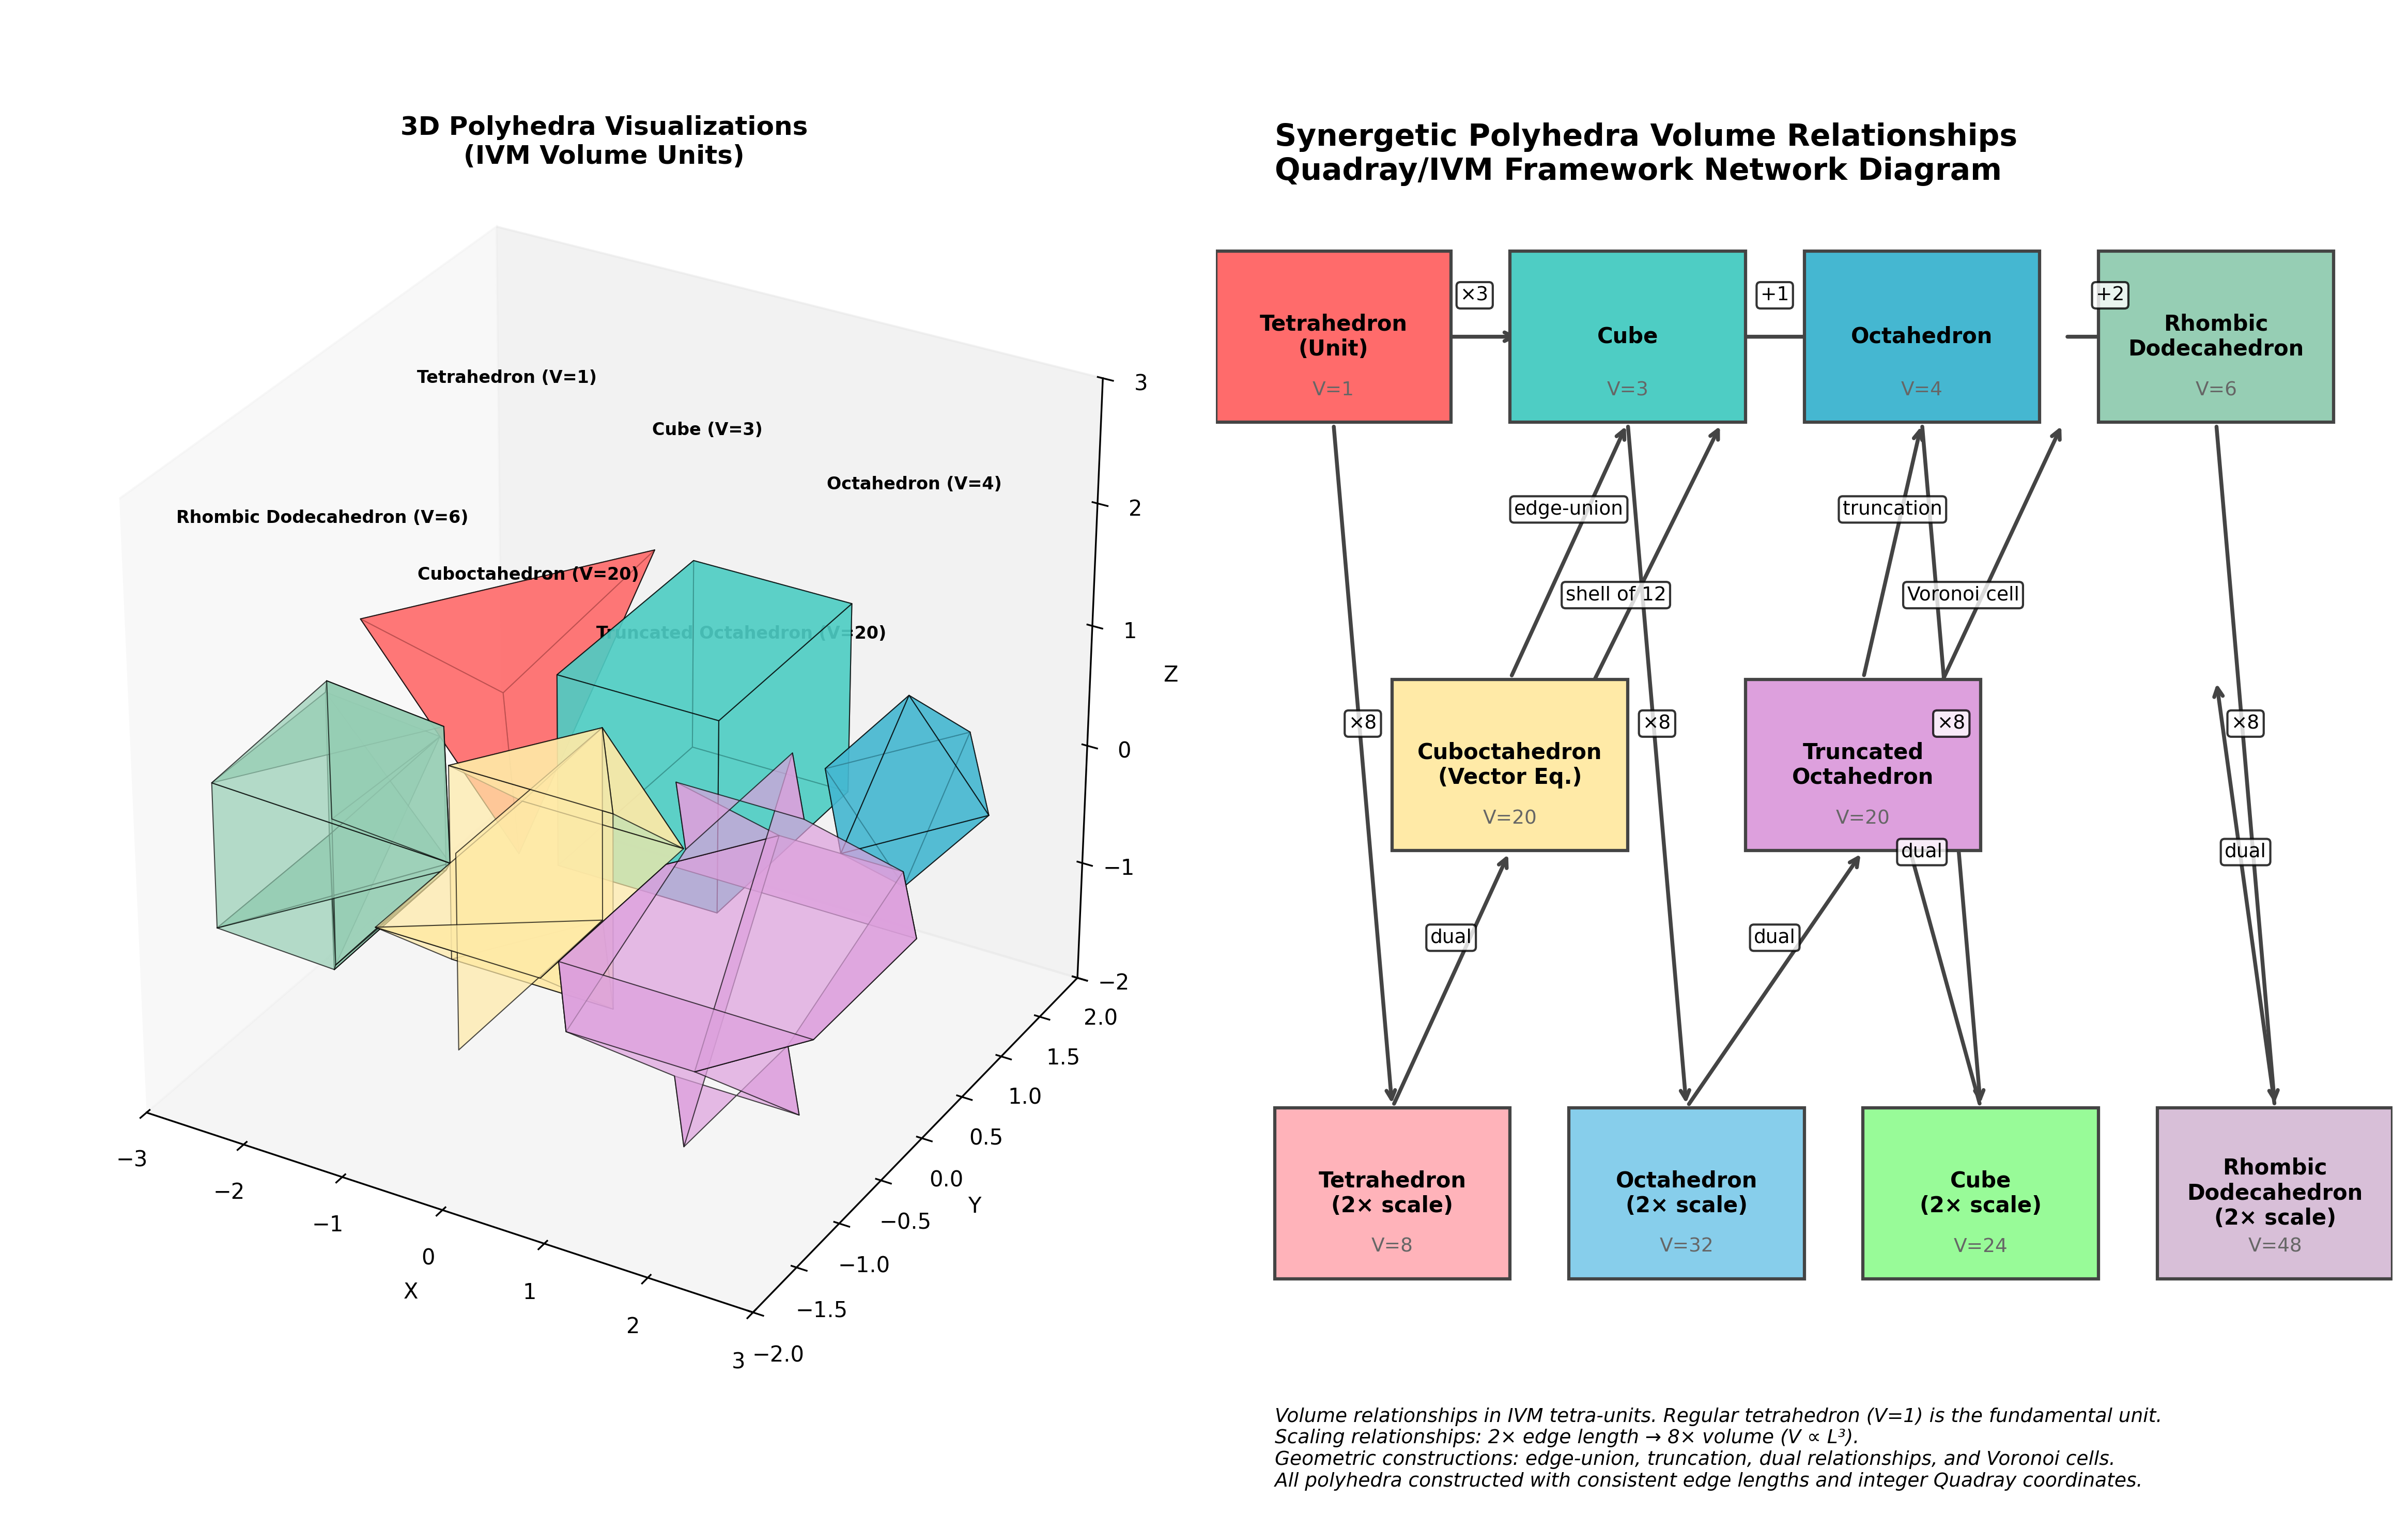
\includegraphics{../output/figures/polyhedra_quadray_constructions.png}
\caption{\textbf{Synergetic polyhedra volume relationships in the
Quadray/IVM framework (comprehensive visualization)}. This figure
combines 3D polyhedra visualizations with an extended network diagram
showing integer volume relationships among key synergetic polyhedra.
\textbf{Left panel (3D visualizations)}: Color-coded polyhedra including
regular tetrahedron (V=1, fundamental unit), cube (V=3), octahedron
(V=4), rhombic dodecahedron (V=6), cuboctahedron (V=20), and truncated
octahedron (V=20), all constructed with consistent edge lengths and
proper geometric faces. \textbf{Right panel (network diagram)}: Extended
volume relationships showing fundamental shapes (V=1,3,4,6), complex
constructions (V=20), and scaling relationships (2× edge length → 8×
volume). \textbf{Additional polyhedra}: Includes truncated octahedron
(V=20) and scaled variants demonstrating the ``third power'' volume
scaling law V ∝ L³ in IVM units. \textbf{Geometric constructions}:
Edge-union relationships, truncation operations, dual polyhedra, and
Voronoi cell constructions. \textbf{Fuller.4D significance}: These
integer volume ratios reflect the quantized nature of space-filling in
synergetics, where the regular tetrahedron provides a natural unit
container and other polyhedra emerge as integer multiples, supporting
discrete geometric computation and exact lattice-based optimization
methods. All constructions respect the IVM unit convention where the
regular tetrahedron has tetravolume 1.}
\end{figure}

\hypertarget{short-python-snippets}{%
\subsubsection{Short Python snippets}\label{short-python-snippets}}

\begin{lstlisting}[language=Python]
from quadray import Quadray, ace_tetravolume_5x5

o = Quadray(0,0,0,0)
p = Quadray(2,1,0,1)
q = Quadray(2,1,1,0)
r = Quadray(2,0,1,1)
assert ace_tetravolume_5x5(o,p,q,r) == 1  # unit IVM tetra
\end{lstlisting}

\begin{lstlisting}[language=Python]
import numpy as np
from cayley_menger import ivm_tetra_volume_cayley_menger

# Example: regular tetrahedron with edge length 1 (XYZ units)
d2 = np.ones((4,4)) - np.eye(4)  # squared distances
V_ivm = ivm_tetra_volume_cayley_menger(d2)   # = 1/8 in IVM tetra-units
\end{lstlisting}

\begin{lstlisting}[language=Python]
# SymPy implementation of Tom Ace 5×5 (symbolic determinant)
from sympy import Matrix

def qvolume(q0, q1, q2, q3):
    M = Matrix([
        q0 + (1,),
        q1 + (1,),
        q2 + (1,),
        q3 + (1,),
        [1, 1, 1, 1, 0],
    ])
    return abs(M.det()) / 4
\end{lstlisting}

\begin{lstlisting}[language=Python]
# Symbolic variant with SymPy (exact radicals)
from sympy import Matrix, sqrt, simplify
from symbolic import cayley_menger_volume_symbolic, convert_xyz_volume_to_ivm_symbolic

d2 = Matrix([[0,1,1,1],[1,0,1,1],[1,1,0,1],[1,1,1,0]])
V_xyz_sym = cayley_menger_volume_symbolic(d2)      # sqrt(2)/12
V_ivm_sym = simplify(convert_xyz_volume_to_ivm_symbolic(V_xyz_sym))  # 1/8
\end{lstlisting}

\hypertarget{random-tetrahedra-in-the-ivm-integer-volumes}{%
\subsubsection{Random tetrahedra in the IVM (integer
volumes)}\label{random-tetrahedra-in-the-ivm-integer-volumes}}

\begin{itemize}
\tightlist
\item
  The 12 CCP directions are the permutations of \((2,1,1,0)\). Random
  walks on this move set generate integer-coordinate Quadrays; resulting
  tetrahedra have integer tetravolumes.
\end{itemize}

\begin{lstlisting}[language=Python]
from itertools import permutations
from random import choice
from quadray import Quadray, ace_tetravolume_5x5

moves = [Quadray(*p) for p in set(permutations((2,1,1,0)))]

def random_walk(start: Quadray, steps: int) -> Quadray:
    cur = start
    for _ in range(steps):
        m = choice(moves)
        cur = Quadray(cur.a+m.a, cur.b+m.b, cur.c+m.c, cur.d+m.d)
    return cur

A = random_walk(Quadray(0,0,0,0), 1000)
B = random_walk(Quadray(0,0,0,0), 1000)
C = random_walk(Quadray(0,0,0,0), 1000)
D = random_walk(Quadray(0,0,0,0), 1000)
V = ace_tetravolume_5x5(A,B,C,D)            # integer
\end{lstlisting}

\hypertarget{algebraic-precision}{%
\subsubsection{Algebraic precision}\label{algebraic-precision}}

\begin{itemize}
\tightlist
\item
  Determinants via floating-point introduce rounding noise. For exact
  arithmetic, use the
  \href{https://en.wikipedia.org/wiki/Bareiss_algorithm}{Bareiss
  algorithm} (already used by
  \passthrough{\lstinline!ace\_tetravolume\_5x5!}) or symbolic engines
  (e.g., \passthrough{\lstinline!sympy!}). For large random-walk
  examples with integer inputs, volumes are exact integers.
\item
  When computing via XYZ determinants, high-precision floats (e.g.,
  \passthrough{\lstinline!gmpy2.mpfr!}) or symbolic matrices avoid
  vestigial errors; round at the end if the underlying result is known
  to be integral.
\end{itemize}

\hypertarget{xyz-determinant-and-the-s3-conversion}{%
\subsubsection{XYZ determinant and the S3
conversion}\label{xyz-determinant-and-the-s3-conversion}}

\begin{itemize}
\tightlist
\item
  Using XYZ coordinates of the four vertices: see Eq. \eqref{eq:xyz_det}
  for the determinant form and the S3 conversion to IVM units.
\end{itemize}

\hypertarget{d3-vs-r3-60-closing-the-lid-vs-orthogonal-cubing}{%
\subsubsection{D\^{}3 vs R\^{}3: 60° ``closing the lid'' vs orthogonal
``cubing''}\label{d3-vs-r3-60-closing-the-lid-vs-orthogonal-cubing}}

\begin{itemize}
\tightlist
\item
  \textbf{IVM (D\^{}3) heuristic}: From a 60--60--60 corner, three
  non-negative edge lengths \(A,B,C\) along quadray directions enclose a
  tetrahedron by ``closing the lid.'' In synergetics, the tetravolume
  scales as the simple product \(ABC\) under IVM conventions (unit
  regular tetra has volume 1). By contrast, in the orthogonal (R\^{}3)
  habit, one constructs a full parallelepiped (12 edges); the tetra
  occupies one-sixth of the triple product of edge vectors. The IVM path
  is more direct for tetrahedra.
\item
  \textbf{Pedagogical note}: Adopt a vector-first approach. Differences
  like \((P_i-P_0)\) denote edge vectors; Quadrays and Cartesian can be
  taught in parallel as vector languages on the same Euclidean
  container.
\end{itemize}

Reference notebook with worked examples and code: See the
\href{07_resources.md}{Resources} section for comprehensive educational
materials and computational implementations.

See implementation:
\passthrough{\lstinline!tetra\_volume\_cayley\_menger!}.

\begin{itemize}
\tightlist
\item
  Lattice projection: round to nearest integer quadray; renormalize to
  maintain non-negativity and a minimal zero.
\end{itemize}

\hypertarget{practical-implementation-workflow}{%
\subsection{Practical Implementation
Workflow}\label{practical-implementation-workflow}}

The methods described in this document follow a unified workflow that
ensures mathematical correctness, computational efficiency, and
reproducibility:

\hypertarget{mathematical-formulation}{%
\subsubsection{1. Mathematical
Formulation}\label{mathematical-formulation}}

\begin{itemize}
\tightlist
\item
  \textbf{Theoretical foundations}: Establish mathematical relationships
  between frameworks (Coxeter.4D ↔ Fuller.4D ↔ Einstein.4D)
\item
  \textbf{Coordinate transformations}: Define linear maps between
  coordinate systems with exact arithmetic
\item
  \textbf{Volume formulations}: Implement multiple approaches (Ace 5×5,
  Cayley--Menger, symbolic) for cross-validation
\end{itemize}

\hypertarget{implementation-strategy-1}{%
\subsubsection{2. Implementation
Strategy}\label{implementation-strategy-1}}

\begin{itemize}
\tightlist
\item
  \textbf{Exact arithmetic}: Use Bareiss algorithm for integer
  determinants, symbolic computation for exact results
\item
  \textbf{Numerical stability}: Implement ridge regularization,
  condition number monitoring, and error handling
\item
  \textbf{Cross-validation}: Ensure different formulations produce
  identical results on test cases
\end{itemize}

\hypertarget{testing-and-validation}{%
\subsubsection{3. Testing and Validation}\label{testing-and-validation}}

\begin{itemize}
\tightlist
\item
  \textbf{Unit tests}: 100\% coverage of all mathematical functions with
  edge case handling
\item
  \textbf{Integration tests}: Validate coordinate transformations and
  volume calculations across frameworks
\item
  \textbf{Numerical validation}: Compare floating-point implementations
  with exact symbolic results
\end{itemize}

\hypertarget{documentation-and-reproducibility}{%
\subsubsection{4. Documentation and
Reproducibility}\label{documentation-and-reproducibility}}

\begin{itemize}
\tightlist
\item
  \textbf{Code-documentation sync}: All mathematical concepts have
  corresponding implementations in \passthrough{\lstinline!src/!}
\item
  \textbf{Figure generation}: Scripts in
  \passthrough{\lstinline!quadmath/scripts/!} generate all figures from
  source code
\item
  \textbf{Data export}: CSV/NPZ files accompany all figures for complete
  reproducibility
\end{itemize}

\hypertarget{optimization-and-extension}{%
\subsubsection{5. Optimization and
Extension}\label{optimization-and-extension}}

\begin{itemize}
\tightlist
\item
  \textbf{Lattice constraints}: Integer volume quantization enables
  discrete optimization methods
\item
  \textbf{Information geometry}: Fisher metric guides natural gradient
  descent on parameter manifolds
\item
  \textbf{Active inference}: Free energy minimization drives both
  perception and action updates
\end{itemize}

This workflow ensures that mathematical theory, computational
implementation, and practical application remain coherent and verifiable
throughout the development process.

\hypertarget{code-methods-anchors}{%
\subsection{Code methods (anchors)}\label{code-methods-anchors}}

\hypertarget{code:core_quadray}{%
\subsubsection{Core Quadray operations}\label{code:core_quadray}}

\hypertarget{code:Quadray}{%
\paragraph{\texorpdfstring{\texttt{Quadray}}{Quadray}}\label{code:Quadray}}

Source: \passthrough{\lstinline!src/quadray.py!} --- Quadray vector
class with non-negative components and at least one zero (Fuller.4D).

\hypertarget{code:DEFAULT_EMBEDDING}{%
\paragraph{\texorpdfstring{\texttt{DEFAULT\_EMBEDDING}}{DEFAULT\_EMBEDDING}}\label{code:DEFAULT_EMBEDDING}}

Source: \passthrough{\lstinline!src/quadray.py!} --- canonical 3×4
symmetric embedding matrix for Quadray to XYZ conversion.

\hypertarget{code:to_xyz}{%
\paragraph{\texorpdfstring{\texttt{to\_xyz}}{to\_xyz}}\label{code:to_xyz}}

Source: \passthrough{\lstinline!src/quadray.py!} --- map quadray to R³
via a 3×4 embedding matrix (Fuller.4D → Coxeter.4D slice).

\hypertarget{code:magnitude}{%
\paragraph{\texorpdfstring{\texttt{magnitude}}{magnitude}}\label{code:magnitude}}

Source: \passthrough{\lstinline!src/quadray.py!} --- return Euclidean
magnitude \textbar\textbar q\textbar\textbar{} under the given embedding
(vector norm).

\hypertarget{code:dot}{%
\paragraph{\texorpdfstring{\texttt{dot}}{dot}}\label{code:dot}}

Source: \passthrough{\lstinline!src/quadray.py!} --- return Euclidean
dot product \textless q1,q2\textgreater{} under the given embedding.

\hypertarget{code:volume_calculations}{%
\subsubsection{Volume calculations}\label{code:volume_calculations}}

\hypertarget{code:integer_tetra_volume}{%
\paragraph{\texorpdfstring{\texttt{integer\_tetra\_volume}}{integer\_tetra\_volume}}\label{code:integer_tetra_volume}}

Source: \passthrough{\lstinline!src/quadray.py!} --- integer 3×3
determinant for lattice tetravolume.

\hypertarget{code:ace_tetravolume_5x5}{%
\paragraph{\texorpdfstring{\texttt{ace\_tetravolume\_5x5}}{ace\_tetravolume\_5x5}}\label{code:ace_tetravolume_5x5}}

Source: \passthrough{\lstinline!src/quadray.py!} --- Tom Ace 5×5
determinant in IVM units.

\hypertarget{code:tetra_volume_cayley_menger}{%
\paragraph{\texorpdfstring{\texttt{tetra\_volume\_cayley\_menger}}{tetra\_volume\_cayley\_menger}}\label{code:tetra_volume_cayley_menger}}

Source: \passthrough{\lstinline!src/cayley\_menger.py!} --- length-based
formula (XYZ units).

\hypertarget{code:ivm_tetra_volume_cayley_menger}{%
\paragraph{\texorpdfstring{\texttt{ivm\_tetra\_volume\_cayley\_menger}}{ivm\_tetra\_volume\_cayley\_menger}}\label{code:ivm_tetra_volume_cayley_menger}}

Source: \passthrough{\lstinline!src/cayley\_menger.py!} ---
Cayley--Menger volume converted to IVM units.

\hypertarget{code:coordinate_conversions}{%
\subsubsection{Coordinate
conversions}\label{code:coordinate_conversions}}

\hypertarget{code:urner_embedding}{%
\paragraph{\texorpdfstring{\texttt{urner\_embedding}}{urner\_embedding}}\label{code:urner_embedding}}

Source: \passthrough{\lstinline!src/conversions.py!} --- canonical XYZ
embedding.

\hypertarget{code:quadray_to_xyz}{%
\paragraph{\texorpdfstring{\texttt{quadray\_to\_xyz}}{quadray\_to\_xyz}}\label{code:quadray_to_xyz}}

Source: \passthrough{\lstinline!src/conversions.py!} --- apply embedding
matrix to map Quadray to XYZ.

\hypertarget{code:linear_algebra}{%
\subsubsection{Linear algebra utilities}\label{code:linear_algebra}}

\hypertarget{code:bareiss_determinant_int}{%
\paragraph{\texorpdfstring{\texttt{bareiss\_determinant\_int}}{bareiss\_determinant\_int}}\label{code:bareiss_determinant_int}}

Source: \passthrough{\lstinline!src/linalg\_utils.py!} --- exact integer
Bareiss determinant.

\hypertarget{code:optimization}{%
\subsubsection{Optimization methods}\label{code:optimization}}

\hypertarget{code:nelder_mead_quadray}{%
\paragraph{\texorpdfstring{\texttt{nelder\_mead\_quadray}}{nelder\_mead\_quadray}}\label{code:nelder_mead_quadray}}

Source: \passthrough{\lstinline!src/nelder\_mead\_quadray.py!} ---
Nelder--Mead optimization adapted to the integer quadray lattice.

\hypertarget{code:discrete_ivm_descent}{%
\paragraph{\texorpdfstring{\texttt{discrete\_ivm\_descent}}{discrete\_ivm\_descent}}\label{code:discrete_ivm_descent}}

Source: \passthrough{\lstinline!src/discrete\_variational.py!} ---
greedy integer-valued descent over the IVM using canonical neighbor
moves; returns a \passthrough{\lstinline!DiscretePath!} with visited
Quadrays and objective values.

\hypertarget{code:neighbor_moves_ivm}{%
\paragraph{\texorpdfstring{\texttt{neighbor\_moves\_ivm}}{neighbor\_moves\_ivm}}\label{code:neighbor_moves_ivm}}

Source: \passthrough{\lstinline!src/discrete\_variational.py!} ---
return the 12 canonical IVM neighbor moves as Quadray deltas.

\hypertarget{code:apply_move}{%
\paragraph{\texorpdfstring{\texttt{apply\_move}}{apply\_move}}\label{code:apply_move}}

Source: \passthrough{\lstinline!src/discrete\_variational.py!} --- apply
a lattice move and normalize to the canonical representative.

\hypertarget{code:information_geometry}{%
\subsubsection{Information geometry
methods}\label{code:information_geometry}}

\hypertarget{code:fisher_information_matrix}{%
\paragraph{\texorpdfstring{\texttt{fisher\_information\_matrix}}{fisher\_information\_matrix}}\label{code:fisher_information_matrix}}

Source: \passthrough{\lstinline!src/information.py!} --- empirical
outer-product estimator.

\hypertarget{code:fisher_information_quadray}{%
\paragraph{\texorpdfstring{\texttt{fisher\_information\_quadray}}{fisher\_information\_quadray}}\label{code:fisher_information_quadray}}

Source: \passthrough{\lstinline!src/information.py!} --- compute Fisher
information matrix in both Cartesian and Quadray coordinates.

\hypertarget{code:natural_gradient_step}{%
\paragraph{\texorpdfstring{\texttt{natural\_gradient\_step}}{natural\_gradient\_step}}\label{code:natural_gradient_step}}

Source: \passthrough{\lstinline!src/information.py!} --- damped
inverse-Fisher step.

\hypertarget{code:free_energy}{%
\paragraph{\texorpdfstring{\texttt{free\_energy}}{free\_energy}}\label{code:free_energy}}

Source: \passthrough{\lstinline!src/information.py!} --- discrete-state
variational free energy.

\hypertarget{code:expected_free_energy}{%
\paragraph{\texorpdfstring{\texttt{expected\_free\_energy}}{expected\_free\_energy}}\label{code:expected_free_energy}}

Source: \passthrough{\lstinline!src/information.py!} --- expected free
energy for Active Inference with prior preferences.

\hypertarget{code:active_inference_step}{%
\paragraph{\texorpdfstring{\texttt{active\_inference\_step}}{active\_inference\_step}}\label{code:active_inference_step}}

Source: \passthrough{\lstinline!src/information.py!} --- joint
perception-action update step in Active Inference.

\hypertarget{code:information_geometric_distance}{%
\paragraph{\texorpdfstring{\texttt{information\_geometric\_distance}}{information\_geometric\_distance}}\label{code:information_geometric_distance}}

Source: \passthrough{\lstinline!src/information.py!} --- compute
information-geometric distance between two points.

\hypertarget{code:perception_update}{%
\paragraph{\texorpdfstring{\texttt{perception\_update}}{perception\_update}}\label{code:perception_update}}

Source: \passthrough{\lstinline!src/information.py!} --- continuous-time
perception update: dμ/dt = D μ - dF/dμ.

\hypertarget{code:action_update}{%
\paragraph{\texorpdfstring{\texttt{action\_update}}{action\_update}}\label{code:action_update}}

Source: \passthrough{\lstinline!src/information.py!} --- continuous-time
action update: da/dt = -dF/da.

\hypertarget{code:finite_difference_gradient}{%
\paragraph{\texorpdfstring{\texttt{finite\_difference\_gradient}}{finite\_difference\_gradient}}\label{code:finite_difference_gradient}}

Source: \passthrough{\lstinline!src/information.py!} --- compute
numerical gradient of a scalar function via central differences.

\hypertarget{code:metrics}{%
\subsubsection{Metrics and analysis}\label{code:metrics}}

\hypertarget{code:shannon_entropy}{%
\paragraph{\texorpdfstring{\texttt{shannon\_entropy}}{shannon\_entropy}}\label{code:shannon_entropy}}

Source: \passthrough{\lstinline!src/metrics.py!} --- Shannon entropy
H(p) for a discrete distribution.

\hypertarget{code:information_length}{%
\paragraph{\texorpdfstring{\texttt{information\_length}}{information\_length}}\label{code:information_length}}

Source: \passthrough{\lstinline!src/metrics.py!} --- path length in
information space via gradient-weighted arc length.

\hypertarget{code:fim_eigenspectrum}{%
\paragraph{\texorpdfstring{\texttt{fim\_eigenspectrum}}{fim\_eigenspectrum}}\label{code:fim_eigenspectrum}}

Source: \passthrough{\lstinline!src/metrics.py!} --- eigen-decomposition
of a Fisher information matrix.

\hypertarget{code:fisher_condition_number}{%
\paragraph{\texorpdfstring{\texttt{fisher\_condition\_number}}{fisher\_condition\_number}}\label{code:fisher_condition_number}}

Source: \passthrough{\lstinline!src/metrics.py!} --- compute the
condition number of the Fisher information matrix.

\hypertarget{code:fisher_curvature_analysis}{%
\paragraph{\texorpdfstring{\texttt{fisher\_curvature\_analysis}}{fisher\_curvature\_analysis}}\label{code:fisher_curvature_analysis}}

Source: \passthrough{\lstinline!src/metrics.py!} --- comprehensive
analysis of Fisher information matrix curvature.

\hypertarget{code:fisher_quadray_comparison}{%
\paragraph{\texorpdfstring{\texttt{fisher\_quadray\_comparison}}{fisher\_quadray\_comparison}}\label{code:fisher_quadray_comparison}}

Source: \passthrough{\lstinline!src/metrics.py!} --- compare Fisher
information matrices between coordinate systems.

\hypertarget{code:examples}{%
\subsubsection{Examples and utilities}\label{code:examples}}

\hypertarget{code:example_ivm_neighbors}{%
\paragraph{\texorpdfstring{\texttt{example\_ivm\_neighbors}}{example\_ivm\_neighbors}}\label{code:example_ivm_neighbors}}

Source: \passthrough{\lstinline!src/examples.py!} --- return the 12
nearest IVM neighbors as permutations of \{2,1,1,0\}.

\hypertarget{code:example_cuboctahedron_neighbors}{%
\paragraph{\texorpdfstring{\texttt{example\_cuboctahedron\_neighbors}}{example\_cuboctahedron\_neighbors}}\label{code:example_cuboctahedron_neighbors}}

Source: \passthrough{\lstinline!src/examples.py!} --- return
twelve-around-one IVM neighbors (vector equilibrium shell).

\hypertarget{code:example_cuboctahedron_vertices_xyz}{%
\paragraph{\texorpdfstring{\texttt{example\_cuboctahedron\_vertices\_xyz}}{example\_cuboctahedron\_vertices\_xyz}}\label{code:example_cuboctahedron_vertices_xyz}}

Source: \passthrough{\lstinline!src/examples.py!} --- return XYZ
coordinates for the twelve-around-one neighbors.

\hypertarget{code:example_partition_tetra_volume}{%
\paragraph{\texorpdfstring{\texttt{example\_partition\_tetra\_volume}}{example\_partition\_tetra\_volume}}\label{code:example_partition_tetra_volume}}

Source: \passthrough{\lstinline!src/examples.py!} --- construct a
tetrahedron from the four-fold partition and return tetravolume.

\hypertarget{code:symbolic}{%
\subsubsection{Symbolic computation}\label{code:symbolic}}

\hypertarget{code:cayley_menger_volume_symbolic}{%
\paragraph{\texorpdfstring{\texttt{cayley\_menger\_volume\_symbolic}}{cayley\_menger\_volume\_symbolic}}\label{code:cayley_menger_volume_symbolic}}

Source: \passthrough{\lstinline!src/symbolic.py!} --- return symbolic
Euclidean tetrahedron volume from squared distances.

\hypertarget{code:convert_xyz_volume_to_ivm_symbolic}{%
\paragraph{\texorpdfstring{\texttt{convert\_xyz\_volume\_to\_ivm\_symbolic}}{convert\_xyz\_volume\_to\_ivm\_symbolic}}\label{code:convert_xyz_volume_to_ivm_symbolic}}

Source: \passthrough{\lstinline!src/symbolic.py!} --- convert a symbolic
Euclidean volume to IVM tetravolume via S3.

\hypertarget{code:visualization}{%
\subsubsection{Visualization and animation}\label{code:visualization}}

\hypertarget{code:animate_discrete_path}{%
\paragraph{\texorpdfstring{\texttt{animate\_discrete\_path}}{animate\_discrete\_path}}\label{code:animate_discrete_path}}

Source: \passthrough{\lstinline!src/visualize.py!} --- animate a
\passthrough{\lstinline!DiscretePath!} to MP4; saves CSV/NPZ trajectory
to \passthrough{\lstinline!quadmath/output/!}.

\hypertarget{code:plot_ivm_neighbors}{%
\paragraph{\texorpdfstring{\texttt{plot\_ivm\_neighbors}}{plot\_ivm\_neighbors}}\label{code:plot_ivm_neighbors}}

Source: \passthrough{\lstinline!src/visualize.py!} --- scatter the 12
IVM neighbor points in 3D.

\hypertarget{code:plot_partition_tetrahedron}{%
\paragraph{\texorpdfstring{\texttt{plot\_partition\_tetrahedron}}{plot\_partition\_tetrahedron}}\label{code:plot_partition_tetrahedron}}

Source: \passthrough{\lstinline!src/visualize.py!} --- plot the
four-fold partition as a labeled tetrahedron in 3D.

\hypertarget{code:animate_simplex}{%
\paragraph{\texorpdfstring{\texttt{animate\_simplex}}{animate\_simplex}}\label{code:animate_simplex}}

Source: \passthrough{\lstinline!src/visualize.py!} --- animate simplex
evolution across iterations.

\hypertarget{code:plot_simplex_trace}{%
\paragraph{\texorpdfstring{\texttt{plot\_simplex\_trace}}{plot\_simplex\_trace}}\label{code:plot_simplex_trace}}

Source: \passthrough{\lstinline!src/visualize.py!} --- plot
per-iteration diagnostics for Nelder--Mead.

\hypertarget{code:utilities}{%
\subsubsection{Path and file utilities}\label{code:utilities}}

\hypertarget{code:get_repo_root}{%
\paragraph{\texorpdfstring{\texttt{get\_repo\_root}}{get\_repo\_root}}\label{code:get_repo_root}}

Source: \passthrough{\lstinline!src/paths.py!} --- heuristically find
repository root by walking up from start.

\hypertarget{code:get_output_dir}{%
\paragraph{\texorpdfstring{\texttt{get\_output\_dir}}{get\_output\_dir}}\label{code:get_output_dir}}

Source: \passthrough{\lstinline!src/paths.py!} --- return
\passthrough{\lstinline!quadmath/output!} path at the repo root and
ensure it exists.

\hypertarget{code:get_data_dir}{%
\paragraph{\texorpdfstring{\texttt{get\_data\_dir}}{get\_data\_dir}}\label{code:get_data_dir}}

Source: \passthrough{\lstinline!src/paths.py!} --- return
\passthrough{\lstinline!quadmath/output/data!} path and ensure it
exists.

\hypertarget{code:get_figure_dir}{%
\paragraph{\texorpdfstring{\texttt{get\_figure\_dir}}{get\_figure\_dir}}\label{code:get_figure_dir}}

Source: \passthrough{\lstinline!src/paths.py!} --- return
\passthrough{\lstinline!quadmath/output/figures!} path and ensure it
exists.

\hypertarget{code:nelder_mead_components}{%
\subsubsection{Additional Nelder--Mead
components}\label{code:nelder_mead_components}}

\hypertarget{code:SimplexState}{%
\paragraph{\texorpdfstring{\texttt{SimplexState}}{SimplexState}}\label{code:SimplexState}}

Source: \passthrough{\lstinline!src/nelder\_mead\_quadray.py!} ---
optimization trajectory state containing vertices, values, volume, and
history.

\hypertarget{code:order_simplex}{%
\paragraph{\texorpdfstring{\texttt{order\_simplex}}{order\_simplex}}\label{code:order_simplex}}

Source: \passthrough{\lstinline!src/nelder\_mead\_quadray.py!} --- sort
vertices by objective value ascending and return paired lists.

\hypertarget{code:centroid_excluding}{%
\paragraph{\texorpdfstring{\texttt{centroid\_excluding}}{centroid\_excluding}}\label{code:centroid_excluding}}

Source: \passthrough{\lstinline!src/nelder\_mead\_quadray.py!} ---
integer centroid of three vertices, excluding the specified index.

\hypertarget{code:project_to_lattice}{%
\paragraph{\texorpdfstring{\texttt{project\_to\_lattice}}{project\_to\_lattice}}\label{code:project_to_lattice}}

Source: \passthrough{\lstinline!src/nelder\_mead\_quadray.py!} ---
project a quadray to the canonical lattice representative via normalize.

\hypertarget{code:compute_volume}{%
\paragraph{\texorpdfstring{\texttt{compute\_volume}}{compute\_volume}}\label{code:compute_volume}}

Source: \passthrough{\lstinline!src/nelder\_mead\_quadray.py!} ---
integer IVM tetra-volume from the first four vertices.

\hypertarget{code:discrete_variational}{%
\subsubsection{Discrete variational
components}\label{code:discrete_variational}}

\hypertarget{code:DiscretePath}{%
\paragraph{\texorpdfstring{\texttt{DiscretePath}}{DiscretePath}}\label{code:DiscretePath}}

Source: \passthrough{\lstinline!src/discrete\_variational.py!} ---
optimization trajectory on the integer quadray lattice.

\hypertarget{code:OptionalMoves}{%
\paragraph{\texorpdfstring{\texttt{OptionalMoves}}{OptionalMoves}}\label{code:OptionalMoves}}

Source: \passthrough{\lstinline!src/discrete\_variational.py!} ---
lightweight protocol for optional typing of moves parameter.

\hypertarget{code:glossary}{%
\subsubsection{Glossary generation}\label{code:glossary}}

\hypertarget{code:build_api_index}{%
\paragraph{\texorpdfstring{\texttt{build\_api\_index}}{build\_api\_index}}\label{code:build_api_index}}

Source: \passthrough{\lstinline!src/glossary\_gen.py!} --- build API
index from source directory.

\hypertarget{code:generate_markdown_table}{%
\paragraph{\texorpdfstring{\texttt{generate\_markdown\_table}}{generate\_markdown\_table}}\label{code:generate_markdown_table}}

Source: \passthrough{\lstinline!src/glossary\_gen.py!} --- generate
markdown table from API entries.

\hypertarget{code:inject_between_markers}{%
\paragraph{\texorpdfstring{\texttt{inject\_between\_markers}}{inject\_between\_markers}}\label{code:inject_between_markers}}

Source: \passthrough{\lstinline!src/glossary\_gen.py!} --- inject
payload between markers in markdown text.

\hypertarget{code:geometry}{%
\subsubsection{Geometry utilities}\label{code:geometry}}

\hypertarget{code:minkowski_interval}{%
\paragraph{\texorpdfstring{\texttt{minkowski\_interval}}{minkowski\_interval}}\label{code:minkowski_interval}}

Source: \passthrough{\lstinline!src/geometry.py!} --- return the
Minkowski interval squared ds² (Einstein.4D).

Relevant tests (\passthrough{\lstinline!tests/!}):

\begin{itemize}
\tightlist
\item
  \passthrough{\lstinline!test\_quadray.py!} (unit IVM tetra,
  divisibility-by-4 scaling, Ace vs.~integer method)
\item
  \passthrough{\lstinline!test\_quadray\_cov.py!} (Ace determinant basic
  check)
\item
  \passthrough{\lstinline!test\_cayley\_menger.py!} (regular tetra
  volume in XYZ units)
\item
  \passthrough{\lstinline!test\_linalg\_utils.py!} (Bareiss determinant
  behavior)
\item
  \passthrough{\lstinline!test\_examples.py!},
  \passthrough{\lstinline!test\_examples\_cov.py!} (neighbors, examples)
\item
  \passthrough{\lstinline!test\_metrics.py!},
  \passthrough{\lstinline!test\_metrics\_cov.py!},
  \passthrough{\lstinline!test\_information.py!},
  \passthrough{\lstinline!test\_paths.py!},
  \passthrough{\lstinline!test\_paths\_cov.py!}
\end{itemize}

\hypertarget{comprehensive-test-coverage}{%
\subsubsection{Comprehensive test
coverage}\label{comprehensive-test-coverage}}

The test suite provides 100\% coverage of all source modules with the
following focus areas:

\hypertarget{core-functionality-tests}{%
\paragraph{Core functionality tests}\label{core-functionality-tests}}

\begin{itemize}
\tightlist
\item
  \textbf{\passthrough{\lstinline!test\_quadray.py!}}: Quadray class
  operations, normalization, volume calculations, vector operations
\item
  \textbf{\passthrough{\lstinline!test\_cayley\_menger.py!}}:
  Cayley--Menger determinant validation, IVM conversion accuracy
\item
  \textbf{\passthrough{\lstinline!test\_linalg\_utils.py!}}: Bareiss
  algorithm correctness, edge cases, numerical stability
\end{itemize}

\hypertarget{optimization-and-variational-methods}{%
\paragraph{Optimization and variational
methods}\label{optimization-and-variational-methods}}

\begin{itemize}
\tightlist
\item
  \textbf{\passthrough{\lstinline!test\_nelder\_mead\_visual.py!}}:
  Nelder--Mead adaptation to quadray lattice, simplex evolution
\item
  \textbf{\passthrough{\lstinline!test\_discrete\_variational.py!}}: IVM
  neighbor moves, discrete descent algorithms, path tracking
\item
  \textbf{\passthrough{\lstinline!test\_active\_inference.py!}}: Free
  energy minimization, perception-action updates
\end{itemize}

\hypertarget{information-geometry-and-metrics}{%
\paragraph{Information geometry and
metrics}\label{information-geometry-and-metrics}}

\begin{itemize}
\tightlist
\item
  \textbf{\passthrough{\lstinline!test\_information.py!}}: Fisher
  information matrix computation, natural gradient steps
\item
  \textbf{\passthrough{\lstinline!test\_metrics.py!}}: FIM
  eigendecomposition, curvature analysis, coordinate system comparisons
\item
  \textbf{\passthrough{\lstinline!test\_information\_cov.py!}}: Extended
  coverage of information geometry functions
\end{itemize}

\hypertarget{examples-and-utilities}{%
\paragraph{Examples and utilities}\label{examples-and-utilities}}

\begin{itemize}
\tightlist
\item
  \textbf{\passthrough{\lstinline!test\_examples.py!}}: IVM neighbor
  constructions, polyhedra volume relationships
\item
  \textbf{\passthrough{\lstinline!test\_examples\_cov.py!}}: Extended
  example function coverage
\item
  \textbf{\passthrough{\lstinline!test\_paths.py!}}: Repository
  structure utilities, output directory management
\end{itemize}

\hypertarget{visualization-and-symbolic-computation}{%
\paragraph{Visualization and symbolic
computation}\label{visualization-and-symbolic-computation}}

\begin{itemize}
\tightlist
\item
  \textbf{\passthrough{\lstinline!test\_visualize.py!}}: Plotting
  functions, animation generation, data export
\item
  \textbf{\passthrough{\lstinline!test\_visualize\_cov.py!}}: Extended
  visualization coverage, edge case handling
\item
  \textbf{\passthrough{\lstinline!test\_symbolic.py!}}: SymPy symbolic
  volume calculations, exact arithmetic
\item
  \textbf{\passthrough{\lstinline!test\_symbolic\_cov.py!}}: Symbolic
  computation error handling
\item
  \textbf{\passthrough{\lstinline!test\_sympy\_formalisms.py!}}:
  End-to-end symbolic workflow validation
\end{itemize}

\hypertarget{api-and-documentation-generation}{%
\paragraph{API and documentation
generation}\label{api-and-documentation-generation}}

\begin{itemize}
\tightlist
\item
  \textbf{\passthrough{\lstinline!test\_glossary\_gen.py!}}: Automatic
  API index generation, markdown table formatting
\item
  \textbf{\passthrough{\lstinline!test\_glossary\_gen\_cov.py!}}:
  Extended glossary generation coverage
\end{itemize}

\hypertarget{reproducibility-checklist}{%
\subsection{Reproducibility checklist}\label{reproducibility-checklist}}

\begin{itemize}
\tightlist
\item
  \textbf{Complete implementation coverage}: All formulas and methods
  discussed in the paper are implemented in
  \passthrough{\lstinline!src/!} modules and verified by comprehensive
  test suites in \passthrough{\lstinline!tests/!}.
\item
  \textbf{Exact arithmetic for integer inputs}: Determinants are
  computed using the Bareiss algorithm for exact integer arithmetic;
  floating-point paths are used only where appropriate and results are
  converted (e.g., via S3) as specified.
\item
  \textbf{Deterministic random experiments}: Random-walk experiments use
  fixed seeds and produce integer volumes; Ace 5×5 determinant agrees
  with length-based methods across all test cases.
\item
  \textbf{Volume tracking and convergence}: Integer simplex volume
  monitoring detects convergence plateaus; face/edge analyses interpret
  sensitivity along edges and enable subspace searches across faces.
\item
  \textbf{Test-driven development}: All source code follows TDD
  principles with 100\% coverage requirements enforced via
  \passthrough{\lstinline!.coveragerc!} configuration.
\item
  \textbf{Figure and data generation}: All figures referenced in
  documentation are generated by scripts in
  \passthrough{\lstinline!quadmath/scripts/!} that import from
  \passthrough{\lstinline!src/!} modules, ensuring code-documentation
  coherence.
\item
  \textbf{Cross-platform compatibility}: Headless matplotlib backend
  (MPLBACKEND=Agg) ensures CI compatibility; deterministic RNG seeds
  guarantee reproducible outputs.
\item
  \textbf{Dependency management}: All dependencies managed through
  \passthrough{\lstinline!uv!} and
  \passthrough{\lstinline!pyproject.toml!} with exact version pinning
  via \passthrough{\lstinline!uv.lock!}.
\item
  \textbf{Path resolution}: No hardcoded paths; all output directories
  resolved via \passthrough{\lstinline!paths.py!} utilities for
  cross-platform compatibility.
\item
  \textbf{Data export formats}: Figures saved alongside CSV/NPZ data for
  complete reproducibility; all generation scripts print output paths
  for manifest collection.
\end{itemize}

All source code, tests, and documentation are available in the
docxology/QuadMath repository, ensuring complete transparency and
reproducibility of the methods described herein.

\end{document}
